\chapter{Extrinsic Evaluation}\label{ch:extrinsiceval}
\section{Introduction}
\label{sec:extrinsic}
The intrinsic evaluation proposed in Chapter~\ref{ch:intrinsiceval} is not based on any particular search task, and thus may not reflect the real utility of the generated facets in assisting search. Therefore, we describe an extrinsic evaluation method which evaluates a system based on an interactive search task that incorporates Faceted Web Search (FWS). We believe the task is similar to a real application of FWS as illustrated in Figure~\ref{fig:fws-example}: a user searches using an under-specified query, the FWS system provides query facets from which the user can select feedback terms that would help further specify the query, after which the FWS system uses the feedback terms for re-ranking documents.

For the extrinsic evaluation, ideally we could ask real users or carry out user studies to try each FWS systems, and measure the gain and cost for using them. The gain can be measured by the improvement of the re-ranked results using standard IR metrics like MAP or nDCG. The cost can be measured by the time spent by the users giving facet feedback. However this evaluation is difficult and expensive to extend for evaluating new systems rapidly.

We instead propose to \emph{simulate} the user feedback process based on a user interaction model, using oracle feedback terms and facet terms collected from annotators. Both the oracle feedback and annotator feedback incrementally select all feedback terms that a user may select, which will then be used in simulation based on the user model to determine which subset of the oracle or annotator feedback terms are selected by a user and how much time is spent giving that feedback. Finally, the systems are evaluated by the re-ranking performance together with the estimated time cost.

For the simulated FWS task, we use the TREC Web track dataset of the diversification task~\cite{clarke2009overview,clarke2010overview,clarke2011overview,clarke2012overview}. It includes query topics that are structured as a representative set of subtopics, each related to a different user need, with relevance judgment made at the subtopic level. In our task, each subtopic is regarded as the search intent of a user, and the corresponding topic title is used as the under-specified query issued to the FWS system. For example, for query number 10 in the TREC 2009 Web Track, the title ``cheap internet'' is used as the initial query, and its subtopic ``I want to find cheap DSL providers'' is regarded as the search intent of the user.

We conduct extrinsic evaluations on combinations of different query facet generation models and facet feedback models in our experiments. We show that by using facet feedback from users, Faceted Web Search is able to assist the search task and significantly improve ranking performance.
Comparing intrinsic evaluation and extrinsic evaluation on different facet generation models, we find that the intrinsic evaluation does not always reflect system utility in real application. Comparing different facet feedback models, we find that the Boolean filtering models, which are widely used in conventional faceted search, are too strict in Faceted Web Search, and less effective than soft ranking models.

In the rest of this Chapter, we first describe how we collect simulated facet feedback in Section~\ref{sec:oa-feedback}. Then, we describe our user model for estimating the feedback time cost to users in Section~\ref{sec:user-model}. Last, we present our experiments for conducting extrinsic evaluation on different faceted web search systems (different combinations of query facet generation models and facet feedback models) in Section~\ref{sec:ee-exp}, followed by conclusions in Section~\ref{sec:ee-conclusions}. 

%The work in this chapter is completed and published~\cite{kong2014extending}.

\section{Oracle and Annotator Feedback} \label{sec:oa-feedback}
Oracle feedback presents an idealized case of facet feedback, in which only \emph{effective} terms -- those that improve the quality of the ranked list -- are selected as feedback terms. We extract oracle feedback terms by testing each single term in the presented facets. Each single candidate term is used by a facet feedback model to re-rank the documents and the candidate term is selected for the oracle if the improvement of the re-ranked documents meets a threshold. In our experiment, we use MAP as the metric and set the threshold to be 0.01. Since we have two types of feedback models, there are two sets of oracle feedback terms --  one uses the Boolean filter models, and one uses the soft ranking models.
%Note that when using a single feedback term, the different feedback models of the same type will have same results, as discussed in Section~\ref{sec:feedback}.

Oracle feedback is cheap to obtain for any facet system (assuming document relevance judgments are available), however it may be quite different from what actual users may select in a real interaction. Therefore, we also collect feedback terms from annotators. Our annotation interface is shown in Figure~\ref{fig:feedback-annotation}. The facet feedback annotation is done by presenting the facets (corresponding to list 1 to 5 in Figure~\ref{fig:feedback-annotation}) to an annotator with description of the information need (corresponding to subtopic description in Figure~\ref{fig:feedback-annotation}) and the initial under-specified query. The annotator is asked to select all the terms from the facets that would help address the information need (corresponding to step 2 in Figure~\ref{fig:feedback-annotation}). Ideally, we could present all the facets generated from different FWS systems for this annotation, but it would be quite expensive. In our experiment, we only present the annotator with facets collected 
from the intrinsic evaluation. This assumes all other facet terms generated by systems are uninteresting to the user or at least not easy for the user to select.

\begin{figure}[H]
\centering
\epsfig{file=figure/feedback-annotation-ui.png,scale=0.55}
%\includegraphics[scale=0.45]{figure/fws-example.png}
\caption{Annotation interface for facet feedback annotation.}
\label{fig:feedback-annotation}
\end{figure}

\section{User Model} \label{sec:user-model}
The user model describes how a user selects feedback terms from facets, based on which we can estimate the time cost for the user. While any reasonable user model can be brought to play here, we use a simple one, similar to the user model others have used for selecting suggestions from clusters of query auto-completions~\cite{jain2010organizing}.

Our user model is based on the structural property of facets. By grouping terms into facets, the facet interface essentially provides a skip list of these facet terms for users. More specifically, in the model, a user sequentially scans presented query facets and skips an entire facet if the user finds the facet irrelevant. Otherwise, the user will scan within the facet, sequentially reading and selecting desired facet terms, until the user finds the desired one or ones. Based on this user model, the time cost for giving facet feedback can be calculated as as,
\begin{equation}
 T(\mathcal{F}^u) = 
\sum_{F^u \in \mathcal{F}^u}{\left( T_f(F^u) + \sum_{t\in ts(F^u)}{T_t(t)} \right)} 
\end{equation}
The righthand side of the equation contains two parts. The first part $T_f(F^u)$ is the time for scanning a facet and deciding relevance, and the second part is the time for scanning/selecting terms in the relevant facets. $ts(F^u)$ is the set of terms scanned/selected in $F^u$'s corresponding query facet, and $T_t(t)$ is the time used for scanning/selecting a term. Since we assume users sequentially scan the terms inside a facet, $ts(F^u)$ will include all the beginning terms in $F^u$'s corresponding facet until the last selected term. This is based on the assumption that users are clear about what terms to select, and stop scanning after finding all of them.
\todo{need to correct the formula}

To simplify the estimation, we further assume time costs are equal for scanning different facets, and equal for scanning/selecting different terms. Then the estimation becomes
\begin{equation}
 T(\mathcal{F}^u) = |\mathcal{F}^u|\cdot T_f + |ts(\mathcal{F}^u)|\cdot T_t
\end{equation}
where $|ts(\mathcal{F}^u)|=\sum_{F^u \in \mathcal{F}^u}{|ts(F^u)|}$ is the total number of term scanned/selected. $T_f$ and $T_t$ are now parameters representing the time for scanning a facet and time for scanning/selecting a term respectively.

To estimate parameters $T_f$ and $T_t$, we tracked annotator behavior during the feedback annotation described in Section~\ref{sec:oa-feedback}, including selecting / un-selecting terms and starting / exiting an annotation session. We only used annotation sessions which did not contain any un-selecting actions, and filtered out some inappropriate sessions, e.g. the annotator dwells for a long time with no activity. This selection results in 274 annotator sessions. We then extracted $|\mathcal{F}^u|$ and $|ts(\mathcal{F}^u)|$ as well as the time cost $T(\mathcal{F}^u)$ for each session, and used linear regression to fit the model to the data. When using sessions from all annotators, $T_f$ and $T_t$ are estimated as 2.60 and 1.60 seconds respectively, with $R^2=0.089$. The low $R^2$ is partly due to the variance introduced by using sessions of different annotators. When using one single annotator we obtain a better fit with $R^2=0.555$, and $T_f=1.51$, $T_t=0.66$, for one of the annotators. Since the 
estimation for $T_f$ is about twice of $T_t$, for simplicity, in our experiment, we set $T_f=2\cdot T_t$, and report the time cost in the time unit of reading/scanning a single term.
\todo{Test $T_f=2\cdot T_t$}

Based on this user model, given oracle/annotator feedback, which represents all the terms that a user may select, the extrinsic evaluation works as follows. We incrementally include each term in oracle/annotator feedback as a feedback terms, and measure how ranking performance changes together with the time cost estimated based on the user model. 

\section{Experiments} \label{sec:ee-exp}
\todo{add an interactive model baseline}
\todo{Call QFI, QFJ consistently}
%In this section, we describes the experiment results for comparing 
\subsection{Experiment Settings}
\textbf{Data set}. For the document corpus, we use the ClueWeb09 Category-B collection and apply spam filtering with a threshold of 60 using the Waterloo spam scores~\cite{cormack2011efficient}. The spam-filtered collection is stemmed using the Krovetz stemmer~\cite{krovetz1993viewing}. For the query topics and subtopics, we used those from TREC Web Track's diversity task from 2009 to 2012, which also contain relevance judgments for documents with respect to each subtopic. We constrain the subtopics to have at least one relevant document in the spam-filtered collection, and this results in 196 queries and 678 query subtopics in our experiment set. For the relevance judgment, any documents that are not in the spam-filtered collection are discarded.

\textbf{Annotation}. We collected facet annotations as described in Section~\ref{sec:ie-data} for all 196 queries. Facets are pooled from the top 10 facets generated by runs from QDM, pLSA, LDA, QFI and QFJ. Then annotators are asked to group the terms in the pool into query facets, and to give a rating for the query facet using a scale of good (2) or fair (1). Facet annotation statistics for the good and fair facets, as well as the pooled facet, are given in Table~\ref{tab:facet-annotations}. The table shows the average number of facet terms per query, average number of query facets per query, and average number of facet terms per facet, for each categories (fair, good, and pooled facets).

\begin{table}[H]
\centering
\caption{Facet annotation statistics}
\label{tab:facet-annotations}
\begin{tabular}{|l|r|r|r|} \hline
& fair & good & pooled\\ \hline
\#terms per query & 15.8 & 26.5 & 240.0\\ 
\#facets per query & 2.3 & 3.8 & 40.9 \\ 
\#terms per facet & 6.8 & 6.9 & 5.9 \\ \hline
\end{tabular}
\end{table}

For the extrinsic evaluation, we also collected facet feedback annotations as described in Section~\ref{sec:extrinsic} for all  678 subtopics. The statistics are given in Table~\ref{tab:feedback-terms}, which also includes statistics for oracle feedback. The table shows the number of feedback terms selected per subtopic and the number of feedback facets per subtopic. For some subtopics, there may be no feedback terms selected, so we also report feedback coverage over subtopics in the table. 
%We can see oracle feedback selects more feedback terms from more facets than annotator feedback, while annotator feedback has slightly higher coverage. 
\begin{table}[H]
\centering
\caption{Oracle and annotator feedback statistics. oracle-b and oracle-s are oracle feedback based on the Boolean filter model and soft ranking model respectively.}
% \label{tab:feedback-terms}
% \begin{tabular}{|c|c|c|c|} \hline
% type & \#t/subtopic & \#f/subtopic & feedback ratio\\ \hline
% annotator & 4.10 & 1.36 & 0.80 \\ \hline
% oracle-b & 7.83 & 2.40 & 0.74 \\  \hline
% oracle-s & 5.24 & 1.93 & 0.72 \\  \hline
% \end{tabular}
\label{tab:feedback-terms}
\begin{tabular}{|c|c|c|c|} \hline
	    & annotator & oracle-b & oracle-s\\ \hline
\#fdbk terms/subtopic & 4.10 & 7.83 & 5.24 \\ \hline
\#fdbk facet/subtopic & 1.36 & 2.40 & 1.93 \\  \hline
feedback coverage &  0.80 & 0.74 & 0.72 \\  \hline
\end{tabular}
\end{table}


\textbf{Training/testing and parameter tuning} are based on 4-fold cross validation for the same splits of the 196 queries.

\textbf{Significance test} is performed by using paired t-test, using 0.05 as the p-value threshold.

\textbf{Facet Generation Models}. We compare pLSA, LDA, QDM, QFI and QFJ. $wPRF$ ($wPRF_{\alpha,\beta}$ with $\alpha$ and $\beta$ set to 1.0) is used as the metric for parameter tuning. For pLSA and LDA, we tune the number of facets and the number of facet terms in a facet. For QDM we tune the two parameters used in the clustering algorithm, the diameter threshold for a cluster and the weight threshold for a valid cluster, as well as the parameters they used for selecting facet terms in each facet. 
%For QFI and QFJ, we do not use the features based on snippets (which was used in previous work~\cite{kong2013extracting}), since snippets are not available in our system. 
For QFI, we tune the weight threshold for facet terms, and the diameter threshold. For QFJ, there are no parameters that need to be tuned.

\textbf{Baseline Retrieval Models and Facet Feedback Models}. We use SDM as the baseline retrieval model with 0.8, 0.15, 0.05 weights for word unigrams, adjacent word bigrams, and adjacent word proximity respectively. SDM is also used as the initial retrieval model for facet generation and facet feedback. We compare different facet feedback models to SDM, including AND, OR, A+O for the Boolean filtering models, as well as ST and SF for the soft ranking models. $\lambda$ in ST/SF is set to be 0.8. Dirichlet smoothing $\mu=1500$ is used for both SDM and ST/SF. We also used other baselines including RM3~\cite{abdul2004umass,lavrenko2001relevance}, a pseudo relevance feedback model, tuned on MAP, and xQuAD~\cite{santos2010exploiting}, a diversification model, tuned on $\alpha$-NDCG~\cite{clarke2008novelty}.
%PM-2~\cite{dang2013term} and

\subsection{Oracle and Annotator Feedback}
%We first compare oracle and annotator feedback, which are the two types of feedback used for simulating user feedback. 
In Figure~\ref{fig:feedback}, we compare the effectiveness of oracle and annotator feedback. It shows how ranking performance changes as time cost increases, when incrementally including terms from the two types of feedback as feedback terms. The time cost is estimated by the user model described in Section~\ref{sec:user-model}. MAP is calculated with respect to the subtopic level relevance, since we are evaluating the case where the user is looking for the subtopic information. MAP value is averaged by macro-averaging -- averaging for subtopics within the same query first, and then across all the queries. \footnote{We also measured micro-averaging, but the results are similar.} When time is zero, no feedback terms are used, which is then just the result for the initial ranking from SDM.
%When there are no feedback terms added at a time cost, the result from most recent time will be used.
\begin{figure}[H]
\centering
\caption{MAP change over time for oracle and annotator feedback, based on annotator facets and SF feedback model. oracle-s and oracle-b are the oracle feedback based on the Boolean filtering model and soft ranking model respectively.}
\label{fig:feedback}
\epsfig{file=figure/cmp-feedback-annotator-ffs-MAP.eps,scale=1}
\end{figure}

In Figure~\ref{fig:feedback}, MAP increases from the SDM baseline result for both oracle and facet feedback, with the oracle ones shown to be far more effective. This shows that annotators are able to identify some useful feedback terms, but are not as effective as the ideal case: it seems people have a hard time knowing which terms are most likely to be successful. We further compare the feedback terms selected in oracle and annotator feedback in Table~\ref{tab:feedback}, which also supports this claim.

\begin{table}[H]
\centering
\caption{Comparing feedback terms in annotator feedback and oracle feedback, using oracle-s as ground truth. This table shows that the annotator selects only 44\% of the effective terms and that only 28\% of the selected terms are effective.}
\label{tab:feedback}
\begin{tabular}{|c|c|c|} \hline
Precision & Recall & F1\\  \hline
0.2817 & 0.4412 & 0.2179 \\ \hline
\end{tabular}
\end{table}

Table~\ref{tab:feedback} shows the overlap between oracle and annotator feedback is low according to F1. However, annotators are able to find almost half of the oracle feedback terms. Other oracle feedback terms are difficult for annotators (or users) to recognize, due to lack of background knowledge, or underlying statistical dependencies between words that are difficult to capture. For example, for the query subtopic, ``find the TIME magazine photo essay Barack Obama's Family Tree'', some names of family members are selected in oracle feedback, but not by the annotator. This is because the annotator is not able to capture the relevant relationship between the names of family members and the photo essay, or simply because the annotator does not know those family members' names.
%Implication from this is one could come up with some models to recognize feedback terms missed by users, to further improve the performance.

\subsection{Comparing Facet Generation Models}
\subsubsection{Intrinsic Evaluation}
To compare intrinsic and extrinsic evaluation, we also report intrinsic evaluation on different facet generation models in Table~\ref{tab:intrinsic}. The table shows QFI and QFJ  outperform other models on the overall measure, wPRF. QFI wins because of high recall of facet terms and high F1 of facet term clustering. For rp-nDCG, QFJ and QDM are more effective. These results are consistent with our previous results in Section~\ref{sec:ie-exp}.  
\begin{table}[H]
\centering
\caption{Intrinsic evaluation of facet generation models.}
\label{tab:intrinsic}
\begin{tabular}{|c|c|c|c|c|c|} \hline
Model & wTP & wTR & wPF & wPRF & rp-nDCG\\ \hline
pLSA & 0.2198 & 0.6273 & 0.2541 & 0.2521 & 0.0561\\ \hline
LDA & 0.2720 & 0.5578 & 0.2345 & 0.2571 & 0.0476\\ \hline
QDM & 0.3253 & 0.4024 & 0.2492 & 0.2688 & 0.0908\\ \hline
QFJ & 0.3525 & 0.4060 & 0.2779 & 0.2836 & 0.1359\\ \hline
QFI & 0.2729 & 0.7363 & 0.3859 & 0.3448 & 0.0825\\ \hline
\end{tabular}
\end{table}

\subsubsection{Extrinsic Evaluation} \label{sec:ee-cmp-facet-extrinsic}
Intrinsic evaluation may not reflect the utility of facets in assisting search. In Figure~\ref{fig:cmp-facet} we evaluate different facet generation models using extrinsic evaluation, by showing how MAP changes as time cost increases, similar to Figure~\ref{fig:feedback}.

\begin{figure}[H]
\centering
\caption{MAP change over time for different facets generation models, based on annotator feedback and SF feedback model.}
\label{fig:cmp-facet}
\epsfig{file=figure/cmp-facet-annotator-ffs-MAP.eps,scale=1.1}
\end{figure}

First, Figure~\ref{fig:cmp-facet} shows all models are able to improve ranking from the baseline, which testifies to the potential of FWS. However, the automatically generated facets are less effective than annotator facets. MAP for annotator facets reaches 0.2 by 10 time units, while the models need much more time, ranging from 27 to 47. Second, QFI is more effective than other models over the entire time span. This is consistent with the intrinsic evaluation. Third, the comparison results for other models are less clear. QFJ and QDM are better than pLSA and LDA before 20 time units, but MAP for pLSA and LDA increases much faster afterwards, and ends at a value similar to QFJ. Comparing these results with Table~\ref{tab:intrinsic}, we find intrinsic metrics do not always reflect utility based on extrinsic evaluation, though the generally better performance of QFI is clear in both.

Another way to compare is to see how many terms in the presented facets are selected by annotators, as shown in Figure~\ref{fig:cmp-facet-term}.
\begin{figure}[H]
\centering
\epsfig{file=figure/cmp-facet-annotator-term.eps,scale=1.1}
\caption{Number of feedback terms selected over time on facets generated by different models, based on annotator feedback.}
\label{fig:cmp-facet-term}
\end{figure}
The figure shows that with annotator facets a (simulated) user needs less time for selecting feedback terms. All the other facet generation approaches are similar to each other, with QDM having slightly more feedback terms at the beginning and QFI having more for the rest. This explains why QFI is the best system run in Figure~\ref{fig:cmp-facet-term} -- for the same time cost, QFI has more feedback terms selected by annotators.

If we switch to using the oracle feedback facets, the difference between different facet generation models and annotator facets are no longer that big, as shown in Figure~\ref{fig:cmp-facet-oracle}. Annotator facets are better at the beginning, but the corresponding MAP stops growing at around 20 time units. We find this is due to there not being so many facets available in the annotator facets. The number of terms and facets presented to users will affect this evaluation. In the plot, when there is not a sufficient supply of facets at some time cost, the results from a smaller time cost are used. That is, if the user runs out of facet terms to consider, performance is stuck where it last left off. 
\begin{figure}[H]
\centering
\epsfig{file=figure/cmp-facet-oracle-ffs-MAP.eps,scale=1.1}
\caption{MAP change over time for different facets generation models, based on oracle feedback and SF feedback model.}
\label{fig:cmp-facet-oracle}
\end{figure}

To validate the comparison in Figure~\ref{fig:cmp-facet} and~\ref{fig:cmp-facet-oracle}, we plot  Figure~\ref{fig:cmp-facet-cum-term} which shows the number of accumulated facet terms in the top facets generated by different models. Figure~\ref{fig:cmp-facet-cum-term} shows all models have a sufficient supply of facet terms for these evaluations. All of them present at least 50 facet terms (on average), which will need at least 50 time units for the user to process. This obviates the concern above. However, the annotator only has on average 42.3 facet terms selected, and therefore comparison at a time larger than that might unfairly penalize the annotator facets. We also notice that the first facet in QFI is very large, and overall QFI has more terms in top facets. Since the results are tuned on wPRF with equal weight for term precision and recall, this suggests it is very likely that too much weight is assigned for recall, and a more balanced weight between wP, wR and wFP should be used in wPRF.

%systems that provide giving more facets/terms will be more likely to have higher score when the allowed time is large. However, this will not affect the comparison when the time is small, or when the systems all present facets that could use that much time.
\begin{figure}[H]
\centering
\caption{Accumulated number of facet terms in top facets generated from different facets generation models.}
\label{fig:cmp-facet-cum-term}
\epsfig{file=figure/cmp-facet-cumTerm.eps,scale=1.1}
\end{figure}

\subsection{Comparing Facet Feedback Models}
We compare different facet feedback models in Figure~\ref{sec:cmp-exp-model}. It shows soft ranking models are more effective than Boolean filter models. AND is too aggressive, which hurts the ranking performance as more and more feedback terms are used. The other two Boolean filtering models, OR and A+O, are similar at the beginning. That is because in the beginning there is only one feedback facet, in which case OR and A+O will be equivalent. As more facet terms are selected, A+O performance decreases. For the two soft ranking model, SF and ST are very close, with SF slightly better as time progresses. 
\begin{figure}[H]
\centering
\epsfig{file=figure/cmp-expansion-annotator-annotator-MAP.eps,scale=1.1}
\caption{MAP change over time for different feedback models, based on annotator facets and annotator feedback.}
\label{sec:cmp-exp-model}
\end{figure}
This comparison suggests that Boolean filter models, AND and A+O, are too strict for FWS, and a soft ranking model is more effective for FWS. This situation is probably because in FWS the mapping between facet term and document is incomplete; a document that does not contain the exact facet term may also be relevant. 

\subsection{Comparison to Baseline Retrieval Models}
\label{sec:ex-rms}
We compare FWS with other baseline retrieval models in Table~\ref{fig:cmp-other}. QFI is used as the FWS system here, with SF as the facet feedback model. Annotator feedback terms are used, which represents a real case (not oracle) of FWS application. 
%We also include results for using annotator facets, to see the performance in an ideal case.
In the table, FWS:10 and FWS:50 are QFI runs allowed 10 and 50 time units for feedback respectively. 

First, the table shows that using annotator feedback, FWS can improve ranking over the initial retrieval model, SDM. FWS also obtains better results than RM3, across all the metrics. It is also better than xQuAD for most metrics. The observations testify to the potential of FWS in assisting search. Last, when allowed more time, the results are further improved as shown by the change from FWS:10 to FWS:50.

\begin{table}[H]
\centering
\caption{Retrieval effectiveness comparison with baselines. FWS:10 and FWS:50 are QFI runs allowed 10 and 50 time units for feedback respectively. Statistically significant differences are marked using the first letter of the retrieval model name under comparison.}
%ANNOTATOR:10 is using annotator facets, allowed 10 time units. 
\label{fig:cmp-other}
\begin{tabular}{|c|l|l|l|} \hline
Model & MAP & MRR & nDCG@10\\ \hline
SDM & 0.1854 & 0.3295 & 0.1997\\ \hline
RM3 & 0.1886 & 0.3124 & 0.2010\\ \hline
xQuAD & 0.1822 & $0.3463^{r}$ & 0.2191\\ \hline
FWS:10 & $0.1918^{s}_{x}$ & $0.3476^{s,r}$ & $0.2145^{s,r}$\\ \hline
%QFI:20 & $0.1994^{s,p}$ & $0.3588^{s,p}$ & $0.2278^{s,p}$\\ \hline 
FWS:50 & $0.2044^{s,r}_{x}$ & $0.3736^{s,r}$ & $0.2357^{s,r}$\\ \hline 

%\hline ANNOTATOR:10 & $0.2003^{s,r}_{x}$ & $0.3671^{s,r}$ & $0.2293^{s,r}$\\ \hline
%ANNOTATOR:20 & $0.2068^{s,r}$ & $0.3744^{s,r}$ & $0.2396^{s,r}$\\ \hline
\end{tabular}
\end{table}

\subsection{Comparison to a Retrieval Model with User Feedback}
Section~\ref{sec:ex-rms} shows that, using user feedback on facets, FWS can provide better ranking than other retrieval models that do not incorporate explicit user feedback. In this section, we want to investigate if FWS is more effective than other retrieval models that incorporate user feedback. For this, we compare FWS with a term relevance feedback model~\cite{koenemann1996case,tan2007term}.

The term relevance feedback model we used is based on RM3~\cite{abdul2004umass,lavrenko2001relevance}, and thus denoted as RM3I (``I'' stands for ``interactive''). RM3I shows the expansion terms from RM3 (terms with high probabilities in the top ranked documents) to a user (or an annotator in our simulation). Then RM3I expands the query only with terms selected by the user in the original RM3 feedback model.

FWS and RM3I are similar in that both of them generate terms for users to select, and then use the selected terms as feedback for re-ranking.  
FWS and RM3I are different from two aspects. First, the terms generated can be different. FWS generates terms based on query facet extraction. RM3I generates terms based on RM3, a pseudo relevance feedback model. Second, the presentation of terms are different. RM3I present the terms as a flat list for the user. FWS groups terms into facets. The facet interface essentially provides a skip list of these terms for users. According to our user model (Section~\ref{sec:user-model}), the user can skip an entire facet if the user finds the facet irrelevant. This saves the user a lot of time in considering the terms inside irrelevant facets.

Our experiment is set up as follows. For term generation, we run RM3 for RM3I with different number of pseudo relevant documents, and report the best result, which is obtained by using top 100 documents (this is also the same setting used in FWS). For FWS, we report results for query facets generated by QFI. For user feedback, same as before, we use annotator feedback terms for both models. For feedback models, FWS uses the SF facet feedback model, RMi3 (as described above) uses the original RM3 model, but only with the selected terms for expansion. For both FWS and RM3I, the weights for the original query and expansion are set to 0.8 and 0.2 respectively. For estimating the time in giving user feedback, we use the user model described in Section~\ref{sec:user-model}. So time cost for FWS is estimated as before. Time cost for RM3I is estimated by assuming the list of feedback terms RM3I presented as a single facet.

We report the results in Table~\ref{fig:ex-rm3i}, which shows how the ranking performance changes in terms of MAP when users invest more and more time in giving feedback for FWS and RM3I. We have two observations here. First, we can see that initially (time < 10 units) RM3I outperforms FWS. This indicates that, compared to FWS, RM3I could rank feedback terms that are more effective in the top of its term list. This observation implies that FWS might be improved by considering similar term ranking models/features as in RM3I. Second, we can see that when users spend more time and scan more terms/facets (time > 10 units), FWS outperforms RM3I. This can be explained by the skip list structure in FWS. When users are looking for more terms to select, the skip list structure in FWS helps users to skip irrelevant terms (in the irrelevant facets), saving them time to consider each of the irrelevant terms one by one. Thus, FWS can achieve similar re-ranking performance in a much shorter time comparing to RM3I.
 
\begin{figure}[H]
\centering
\includegraphics[width=0.7\columnwidth]{figure/cmp-prm-annotator-ffs-MAP.eps}
\caption{MAP change over time for FWS and RM3I (RM3 with user feedback terms). Results are based on annotator feedback terms. FWS results are based on QFI.}
\label{fig:ex-rm3i}
\end{figure}

\subsection{Examples}
In this section, we use some system generated facets as examples, to show how FWS can assist search. We find FWS can be helpful in exploratory search. 
For example, for the query ``cheap internet'', the facets generated by QDM includes a facet of different Internet service types, \{\textit{dial up}, \textit{dsl}, \textit{cable}\}, and a facet of different ISPs, \{\textit{netzero}, \textit{juno}, \textit{copper}, \textit{toast}\}. These facets can assist the user to compare different Internet service types and ISPs during his/her exploration of ``cheap Internet''. Another example is the query ``lymphoma in dogs'', in which the user may want to learn about different aspects of lymphoma in dogs. QFJ generates the facet \{\textit{treatment}, \textit{diagnosis}, \textit{prognosis}, \textit{symptoms}, ...\} which represents different aspects of the query. For this query, there is a query subtopic looking for symptoms of lymphoma in dogs, which can be directly answered by another facet found by QFJ, \{\textit{vomiting}, \textit{diarrhea}, \textit{weight loss}, \textit{depression}, \textit{fever}\}. 


\section{Summary} 
\label{sec:ee-conclusions}
In this chapter, we developed an extrinsic evaluation method for Faceted Web Search. The extrinsic evaluation method directly measures the utility in search instead of comparing system/annotator facets as in intrinsic evaluation. We described a way to build reusable test collection for the extrinsic evaluation, and make our collected data set publicly available\footnote{See http://ciir.cs.umass.edu/downloads}.

We also investigated different facet generation and facet feedback models based on the extrinsic evaluation method.
Our experiments show, by using facet feedback from users, Faceted Web Search is able to assist the search task and significantly improve ranking performance. Our experiments also show that the skip list structure in the facet interface helps users save time in considering feedback terms in irrelevant facets. Comparing intrinsic evaluation and extrinsic evaluation on different facet generation models, we find that the intrinsic evaluation does not always reflect system utility in real application. Comparing different facet feedback models, we find that the Boolean filtering models, which are widely used in conventional faceted search, are too strict in Faceted Web Search, and less effective than soft ranking models.
